\section{Design of Recluse}
\label{sec:Recluse}
In this section, we firstly introduce the principle of Recluse with the design goals and main process phases.
Then, we describe the system initialization and initial registration of RP, following with the description of algorithms for calculating the RP identifier transformation, user identifier and account.
The detailed processing for each user's login is provided corresponding to the main process phases.
Finally, we present that Recluse is compatible with OIDC.

\subsection{Principle}
\label{subsec:overview}
\noindent\textbf{Goals in Recluse.}
As analyzed in Section~\ref{subsec:solutions}, Recluse needs to provide trapdoor identification, transformed binding and user-centric confidentiality,
to achieve the privacy-preserving identification, binding and confidentiality.
While, the integrity is provided based on the signature inherited from existing SSO systems.
%to comfort the privacy-preserving requirements of SSO systems, Recluse has to allow only the exact RP to derive the user's unchanged account with a trapdoor, bind the proof with a transformation of RP’s identifier, and achieve user-centric confidentiality of the identity proof.
We %further divide these three requirements into three goals and
achieve these three requirements (goals) using five phases as described in Figure~\ref{fig:Recluse}.
To make the description clear, we list the used notations  in Table~\ref{tbl:notations}.
\begin{itemize}
 \item Generating a self-verifying value for each RP, to provide the correct information for the user-centric check.
  In Recluse, each RP applies a certificate ($Cert_{RP}$) in the \emph{RP initial registration} phase (Steps a and b in Figure~\ref{fig:Recluse}),
  and sends it to the user in each login processing,
  to provide the exact information for  correct construction and transmission of identity proof,
             and therefore achieving \textbf{User-centric Confidentiality}.
  %self-verifying value for the user-centric check (for \textbf{User-centric Confidentiality}),
  % to ensure the correct construction and transmission of identity proof,
  %which is achieved in RP initial registration (step a, b in Figure~\ref{fig:Recluse}), applying for a RP certificate ($Cert_{RP}$), a self-verifying value;




    \item Transforming the RP identifer, to bind the identity proof with the unique RP identifier transformation.  
  In Recluse, the RP and user corporately negotiate a transformation (denoted as $PRPID$) of RP's original identifier (denoted as $RPID$), in the \emph{RP identifier transforming} phase (Step 2.1 in Figure~\ref{fig:Recluse}). 
  IdP checks the uniqueness of $RPID$ in the \emph{dynamic registration} phase (Step 2.2 in Figure~\ref{fig:Recluse}),  to avoid one identity proof being accepted by two or more RPs.
  Then, IdP  binds the identity proof with the unique $PRPID$, and  can never infer $RPID$ from $PRPID$, 
   therefore achieving \textbf{Transformed Binding}.
  %Providing a RP identifier transformation (for \textbf{Transformed Binding}), 
  %to ensure the security by binding the identity proof with this transformation, 
  %and preserve user's privacy by preventing the IdP from inferring the original RP identifier from this transformation in the request, 
  %achieved in RP identifier transforming (step 2.1 in Figure~\ref{fig:Recluse}) generating transformation (denoted as $PRPID$) of RP's original identifier (denoted as $RPID$);
  
  \item Providing algorithms for calculating the user's identifier ($PUID$) in identity proof and the user's account ($Account$) at the RP,
   to allow the RP to identify the user.
   %different $PUID$ generated for different RPs, while a unique $Account$ derived at the RP with the trapdoor.
  In Recluse, IdP calculates $PUID$ based on $PRPID$ and user's unique identifier ($UID$) in the \emph{$PUID$ generation} phase (Step 4 in Figure~\ref{fig:Recluse}), which results in different $PUID$  for different RPs;
  and,  the RP derives the user's unique $Account$  from $PUID$ with the  trapdoor, i.e., the secret parameters of the RP identifier transformation,   in the \emph{$Account$ processing} phase (Step 6 in Figure~\ref{fig:Recluse});
   therefore, achieving \textbf{Trapdoor Identification}.
   %\item 3. Checking the uniqueness of the transformation (for \textbf{Transformed Binding}), to avoid one identity proof being accepted by two or more RPs, which will harm the security of SSO systems, achieved in Dynamic registration (step 2.2 in Figure~\ref{fig:Recluse}), checking the global uniqueness of $RPID$;

 % \item Unlinkable PUID (for \textbf{Trapdoor Identification}), for one user, the $PUID$s for different RPs should vary, to prevent identity linkage, which is achieved in $PUID$ generation (step 4 in Figure~\ref{fig:Recluse}), generating $PUID$ at the IdP, and transferring $PUID$ to the RP;
 % \item Unchanged account (for \textbf{Trapdoor Identification}), to allow only the destination RP (with the trapdoor) to derive the unchanged account for one user from varying $PUID$s, which is necessary for providing the consecutive and individual services, achieved in $Account$ verifying (step 6 in Figure~\ref{fig:Recluse}), calculating the user's account in the RP.

  
   
\end{itemize}

%The core factor in Recluse is the transformation of RP identifier and pairwise user identifier generation which is described detailedly in Section~\ref{subsec:identifier-generation}. 
%$PRPID$ is the transformed RP identifier transmitted to IdP based on the $RPID$ (presenting the unique identity of RP), an one-time random number $N$ and the large prime number $p$ ($RPID$ is the primitive root of $p$) in the function $PRPID = {RPID}^{N} \ mod \ p$. 
%$PUID$ is the user identifier provided by IdP to RP, which is generated in the function $PUID = {PRPID}^{UID} \ mod \ p$ where $UID$ is the unique user identifier stored and only known by IdP. 
%The non-derivability of $RPID$ and $UID$ is based on the Discrete Logarithm Problem.

Discrete logarithm problem is adopted in Recluse, to prevent IdP from inferring $RPID$ from $PRPID$, and allow the RP to derive $Account$ from $PUID$ without obtaining the $UID$. 
Here, we provide a brief description of the discrete logarithm problem.
A number $g$ ($0<g<p$) is called a primitive root modular a prime $p$, if for ${\forall}y$ ($0<y<p$), there is a  number $x$ ($0\le x <p-1$) satisfying $y=g^x \pmod p$. 
And, $x$ is called the discrete logarithm of $y$ modulo $p$. Given a large prime $p$ and a number $y$, it is computationally infeasible to derive the discrete logarithm (here $x$) of $y$ (detailed in~\cite{WXWM}), which is called  Discrete Logarithm Problem. The hardness of solving discrete logarithm has been a base of the security of several security primitives, including Diffie-Hellman key exchange and Digital Signature Algorithm.

\subsection{System Initialization and RP Initial Registration}
In Recluse, the IdP needs to be initialized during the IdP setup, for generating the public parameters for the users and RPs; the RP has to perform only one initial registration at the RP setup; and  the user triggers the Step 2-6 in Figure~\ref{fig:Recluse} for each login at a RP. IdP setup is performed at the very beginning of Recluse, and will be invoked by the IdP to update the leaked $SK_{Cert}$ or $SK_{ID}$, while $g$ and $p$ will never be modified. Recluse does not support multiple initial registrations for one RP, as the RP does not know the $UID$ nor the discrete logarithm of $RPID$ and fails to derive the user's new account from the old one under the Discrete Logarithm problem.


\begin{table}[tb]
    \caption{The notations used in Recluse.}
    \centering
    \begin{tabular}{|c|c|}
    \hline
    {Notation} & {Definition} \\
    \hline
    {$p$} & {A large prime.} \\
    \hline
    {$g$} & {A primitive root  modulo $p$.} \\
    \hline
    {$Cert_{RP}$} & {An RP certificate.} \\
    \hline
    {$SK_{Cert}$, $PK_{Cert}$} & {The private / public key for $Cert_{RP}$.} \\
    \hline
    {$SK_{ID}$, $PK_{ID}$} & {The private / public key for  identity proof.} \\
    \hline
    {$UID$} & {User's unique identifier at IdP.} \\
    \hline
    {$PUID$} & {User's privacy-preserving id in the identity proof.} \\
    \hline
    {$Account$} & {User's identifier at an RP.} \\
    \hline
    {$RPID$} & {RP's original identifier.} \\
    \hline
    {$PRPID$} & {The privacy-preserving $RPID$.} \\
    \hline
    {$n_u$} & {User-generated random nonce for $PRPID$. } \\
    \hline
    {$n_{RP}$} & {RP-generated random nonce for $PRPID$. } \\
    \hline
    {$Y_{RP}$} & {Public value for $n_{RP}$, $(RPID)^{n_{RP}} \ mod p$. } \\
    \hline
    {$t$} & {A trapdoor, $t=(n_u*n_{RP})^{-1} mod \ (p-1)$. } \\
    \hline
    \end{tabular}
    \label{tbl:notations}
\end{table}

\noindent\textbf{IdP Setup.} In the setup, the IdP generates two random asymmetric key pairs, ($PK_{ID}$, $SK_{ID}$) and ($PK_{Cert}$, $SK_{Cert}$), for calculating the signatures in the identity proof and $Cert_{RP}$, respectively; and provides $PK_{ID}$ and $PK_{Cert}$ as the public parameters for the verification of identity proof and $Cert_{RP}$. Moreover, IdP generates a strong prime $p$, calculates  a primitive root ($g$), and provides $p$ and $g$ as the public parameters. For $p$, we firstly randomly choose a large prime $q$, and accept  $2q+1$ as $p$ if $2q+1$ is a prime. The strong prime $p$ makes it easier to choose $n_{u}$ and $n_{RP}$. %With $g$, we obtain all the integers less than $p$, by calculating $g^i mod \ P$ for $0 \leq i \leq (P-1)$.
The IdP setup and following RP initial registration are based on the features of primitive root.

\noindent\textbf{Primitive Root.} To calculate the primitive root for a given large prime $p$,  we first search the least primitive root $g_m$  mod $p$, and then calculate the primitive root $g = g_{m}^{t} mod \ P$, where $t$ is an integer coprime to $p-1$.
We checks whether a integrity $\mu$ is the primitive root modulo $p$ where $p=2q+1$ ($q$ is a prime), based on the lemma that an integer $1<\mu <p-1$ is a primitive root if and only if $\mu^2\neq 1 \pmod p$ and $\mu^q\neq 1 \pmod p$.
The details are provided in~\cite{Shoup,Wang}.


\noindent\textbf{RP Initial Registration.} The RP invokes initial registration to apply a valid and self-verifying $Cert_{RP}$ from IdP (\textbf{Goal 1})
% as provided in Figure~\ref{fig:registration}
, which contains three steps:

\begin{itemize}
\item 1. RP sends IdP a $Cert_{RP}$ request $Req_{Cert_{RP}}$, which contains the distinguished name $Name_{RP}$ (e.g., DNS name) and the endpoint to receive the identity proof.
\item 2. IdP calculates $RPID = g^r mod \ p$ with a random chosen $r$ which is coprime to $p-1$ and different from the ones for other RPs,  generates the signature ($Sig_{SK_{Cert}}$) of [$RPID, Name_{RP}$] using $SK_{Cert}$, and returns [$RPID, Name_{RP}, Sig_{SK_{Cert}}$] as $Cert_{RP}$.
\item 3. IdP sends $Cert_{RP}$ to the RP who verifies $Cert_{RP}$ using $PK_{Cert}$.
\end{itemize}

%\begin{figure}
%  \centering
%  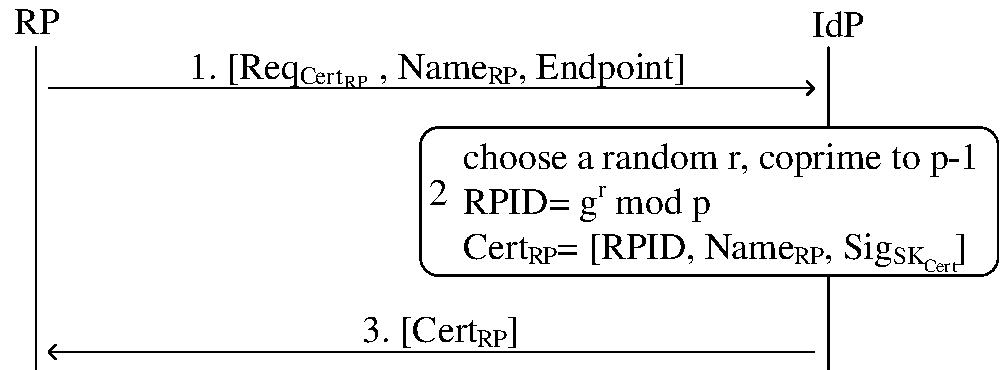
\includegraphics[width=\linewidth]{fig/registration.pdf}
%  \caption{RP initial registration.}
%  \label{fig:registration}
%\end{figure}

%1. r which is coprime to $P-1$来保证$RPID$是一个本原根,从而保证adversary无法从PID中获取UID, ---
%2. $RPID$不能相同,保证RP无法进行identity linkage。 ---RP可以借助类似CT的方案来保证, 没有两个合法证书被颁发给同一个RPID
Here, we further explain the two requirements in the generation of $RPID$ for \textbf{Goal 4}:
\begin{itemize}
  \item $r$ should be coprime to $p-1$. This makes $RPID$ be another primitive root, and satisfies the requirement of Discrete Logarithm problem to prevent the RP inferring $UID$ from $Account$.
  \item $r$ should be different with the ones for other RPs. Otherwise, the RPs who are assigned the same $RPID$, obtain the same $PUID$ for a user, which makes identity linkage possible.
\end{itemize}

The honest IdP is assumed to generate the correct $RPID$. However, we may perform an external check on $Cert_{RP}$ and $RPID$, based on the idea of Certificate transparency. The external check needs to be performed by a third party instead of RP who will be able to perform identity linkage with incorrect $RPID$. To perform the external check, IdP is required to provide the $Cert_{RP}$ to a log server, while a monitor checks the correctness of $Cert_{RP}$, i.e., no two valid $Cert_{RP}$ assigned to a same $RPID$ and $RPID$ is a primitive root modulo $p$. Moreover, $Cert_{RP}$ is compatible with a X.509 certificate which is discussed in Section~\ref{sec:discussion}.




\begin{comment}
\subsection{Primitive Root}
\label{subsec:primitive}
A number $g$ ($0<g<P$) is called a primitive root modular a prime $p$, if for ${\forall}y$ ($0<y<P$), there is a (unique) number $x$ ($0\le x <P-1$) satisfying $y=g^x \pmod P$. Here, $x$ is called the discrete logarithm of $y$ modulo $p$. Given a large prime $p$ and a number $y$, it is computationally infeasible to derive the discrete logarithm (here $x$) of $y$ (detailed in~\cite{WXWM}), which is called  Discrete Logarithm Problem. The hardness of solving discrete logarithm has been a base of the security of several security primitives, including
Diffie-Hellman key exchange and Digital Signature Algorithm.

To calculate the primitive root for a given large prime $p$,  we first search the least primitive root $g_m$  mod $p$, and then calculate the primitive root $g = g_{m}^{t} mod \ P$, where $t$ is an integer coprime to $P-1$.
We checks whether a integrity $\mu$ is the primitive root modulo $p$ where $P=2Q+1$ ($Q$ is a prime), based on the lemma that an integer $1<\mu <P-1$ is a primitive root if and only if $\mu^2\neq 1 \pmod P$ and $\mu^Q\neq 1 \pmod P$.
The details are provided in~\cite{Shoup,Wang}.

\subsection{Overview}
\label{subsec:overview}
\begin{figure}
  \centering
  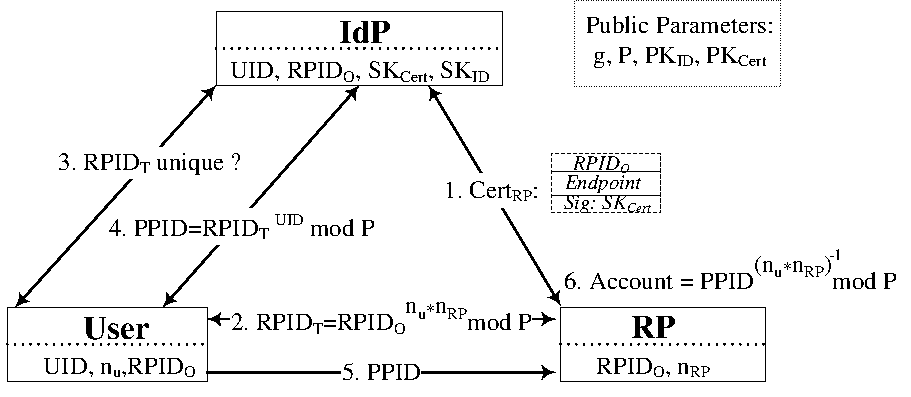
\includegraphics[width=\linewidth]{fig/Overview.pdf}
  \caption{Overview of Recluse.}
  \label{fig:overview}
\end{figure}

\subsection{Goals}
As analyzed in Section~\ref{subsec:solutions}, to enhanced requirements of SSO systems, Recluse has to allow only the exact RP to derive the user's unchanged account with a trapdoor, bind the proof with a transformation of RP’s identifier, and achieve user-centric confidentiality of the identity proof. We further divide these three requirements into 5 goals and achieve these 5 goals using 5 phases which is formed as the process flow in Recluse:
\begin{itemize}
  \item 1. Providing a self-verifying value for the user-centric check (for \textbf{User-centric Confidentiality}), to ensure the correct construction and transmission of identity proof (i.e., user-centric confidentiality), which is achieved in RP initial registration (step a, b in Figure~\ref{fig:overview}), applying for a RP certificate ($Cert_{RP}$), a self-verifying value;
  \item 2. Providing a RP identifier transformation (for \textbf{Transformed Binding}), to ensure the security by binding the identity proof with this transformation, and preserve user's privacy by preventing the IdP from inferring the original RP identifier from this transformation in the request, achieved in RP identifier transforming (step 2.1 in Figure~\ref{fig:overview}) generating transformation (denoted as $PRPID$) of RP's original identifier (denoted as $RPID$);
  \item 3. Checking the uniqueness of the transformation (for \textbf{Transformed Binding}), to avoid one identity proof being accepted by two or more RPs, which will harm the security of SSO systems, achieved in Dynamic registration (step 2.2 in Figure~\ref{fig:overview}), checking the global uniqueness of $RPID$;
  \item 4. Unlinkable PUID (for \textbf{Trapdoor-existing Identification}), for one user, the PUIDs for different RPs should vary, to prevent identity linkage, which is achieved in $PUID$ generation (step 4 in Figure~\ref{fig:overview}), generating PUID at the IdP, and transferring PUID to the RP;
  \item 5. Unchanged account (for \textbf{Trapdoor-existing Identification}), to allow only the destination RP (with the trapdoor) to derive the unchanged account for one user from varying PUIDs, which is necessary for providing the consecutive and individual services, achieved in $Account$ verifying (step 6 in Figure~\ref{fig:overview}), calculating the user's account in the RP.
\end{itemize}

As analyzed in Section~\ref{subsec:solutions}, to ensure the security and privacy of SSO systems, Recluse has to achieve user-centric confidentiality of the identity proof, bind the proof with a transformation of RP’s identifier, and allow only the exact RP to derive the user's unchange account with a trapdoor. We further divide these three solutions into 5 goals to be achieved in the design in Recluse:
\begin{itemize}
  \item 1. Providing a self-verifying value for the user-centric check, to ensure the correct construction and transmission of identity proof (i.e., user-centric confidentiality);
  \item 2. Providing a RP identifier transformation, to ensure the security by binding the identity proof with this transformation, and preserve user's privacy by preventing the IdP from inferring the original RP identifier from this transformation in the request;
  \item 3. Checking the uniqueness of the transformation, to avoid one identity proof being accepted by two or more RPs, which will harm the security of SSO systems;
  \item 4. Unlinkable PUID, for one user, the PUIDs for different RPs should vary, to prevent identity linkage. The $PUID$ is generated at the IdP, and transferred to the RP.
  \item 5. Unchange account, to allow only the destination RP (with the trapdoor) to derive the unchanged account for one user from varying PUIDs, which is necessary for providing the consecutive and individual services.
\end{itemize}

%To hide the user's traces from both the IdP and colluded RPs without breaking the security, Recluse has to achieve these : (1) the user and RP corporately calculate a transformation of the RP's identifier based on Discrete Logarithm Problem, which is sent to the IdP for binding with the identity proof while preventing the IdP from inferring the original RP identifier. The PIDs (in the identity proof) for a user in various RPs are different, to avoid the identity linkage. Moreover, only the RP (and the user) can calculate the trapdoor of the transformation, to transfer the PID into a unchanged account for the user.


Recluse achieves these 5 goals using 5 phases as described in Figure~\ref{fig:overview}, while the used notations are listed in Table~\ref{tbl:notations}. The details are as follows, and the step refers to the one in Figure~\ref{fig:overview}:
\begin{itemize}
  \item RP initial registration: Applying for a RP certificate ($Cert_{RP}$), a self-verifying value,  (Step 1, Goal 1);
  \item RP identifier transforming: Generating transformation (denoted as $RPID_T$) of RP's original identifier (denoted as $RPID$), (Step 2, Goal 2);
  \item Dynamic registration: Checking the global uniqueness of $PRPID$, (Step 3, Goal 3);
  \item PID:  Generating PID at the IdP, and transferring PID to the RP, (Step 4 and 5, Goal 4);
  \item Account: Calculating the user's account in the RP, (Step 6, Goal 5).
\end{itemize}

A RP certificate (denoted as $Cert_{RP}$) is the self-verifying value required in Goal 1, which is  generated in the \textbf{RP initial registration} (phase 1). A transformation (denoted as $PRPID$) of RP's original identifier (denoted as $RPID$) is generated in the \textbf{RP identifier transforming} (phase 2) for Goal 2. The global uniqueness of $PRPID$ is checked in the \textbf{dynamic registration} (phase 3) for Goal 3. The unlinkable \textbf{PID} is generated and transmitted to RP in the step 4 and 5 in Figure~\ref{fig:overview}, for Goal 4.

To achieve these goals, Recluse contains the following 6 phases, in which the IdP setup needs to be executed only once for a IdP, RP initial registration  needs to be invoked only once for a RP, while all the other phases will be invoked repeatedly for each user's login request at each RP. To make the decryption of Recluse clear, we list
\begin{itemize}
  \item IdP setup: Generating correct public parameters;
  \item RP initial registration: Applying RP certificate (denoted as $Cert_{RP}$) from IdP (Step 1 in Figure~\ref{fig:overview});
  \item RP identifier transforming: Generating transformation (denoted as $PRPID$) of RP's original identifier (denoted as $RPID$) (Step 2 in Figure~\ref{fig:overview});
  \item Dynamic registration: Checking the global uniqueness of $PRPID$ (Step 3 in Figure~\ref{fig:overview});
  \item PID:  Generating PID at the IdP, and transferring PID to the RP (Step 4 and 5 in in Figure~\ref{fig:overview});
  \item Account:  Calculating the user's account in the RP (Step 6 in Figure~\ref{fig:overview}).
\end{itemize}

In Recluse, the IdP needs to be initialized during the IdP setup, for generating the public parameters for the users and RPs; the RP has to perform only one initial registration at the RP setup; and  the user triggers the Step 2-6 in Figure~\ref{fig:overview} for each login at a RP. IdP setup is performed at the very beginning of Recluse, and will be invoked by the IdP to update the leaked $SK_{Cert}$ or $SK_{ID}$, while $g$ and $p$ will never be modified. Recluse does not support multiple initial registrations for one RP, as the RP does not know the $UID$ nor the discrete logarithm of $RPID$ and fails to derive the user's new account  from the old one under the Discrete Logarithm problem.


\begin{table}[tb]
    \caption{The notations used in Recluse.}
    \centering
    \begin{tabular}{|c|c|}
    \hline
    {Notation} & {Definition} \\
    \hline
    {$p$} & {A large prime.} \\
    \hline
    {$g$} & {A primitive root  modulo $p$.} \\
    \hline
    {$Cert_{RP}$} & {A RP certificate.} \\
    \hline
    {$SK_{Cert}$, $PK_{Cert}$} & {The private / public key for $Cert_{RP}$.} \\
    \hline
    {$SK_{ID}$, $PK_{ID}$} & {The private / public key for  identity proof.} \\
    \hline
    {$UID$} & {User's unique identifier at IdP.} \\
    \hline
    {$PUID$} & {User's privacy-preserving id in the identity proof.} \\
    \hline
    {$Account$} & {User's identifier at a RP.} \\
    \hline
    {$RPID$} & {RP's original identifier.} \\
    \hline
    {$PRPID$} & {The privacy-preserving $RPID$.} \\
    \hline
    {$n_u$} & {User-generated random nonce for $PRPID$. } \\
    \hline
    {$n_{RP}$} & {RP-generated random nonce for $PRPID$. } \\
    \hline
    {$Y_{RP}$} & {Public value for $n_{RP}$, $(RPID)^{n_{RP}} \ mod P$. } \\
    \hline
    {$t$} & {A trapdoor, $t=(n_u*n_{RP})^{-1} mod \ (P-1)$. } \\
    \hline
    \end{tabular}
    \label{tbl:notations}
\end{table}

\noindent\textbf{IdP setup.} In the setup, the IdP generates two random asymmetric key pairs, ($PK_{ID}$, $SK_{ID}$) and ($PK_{Cert}$, $SK_{Cert}$), for calculating the signatures in the identity proof and $Cert_{RP}$, respectively; and provides $PK_{ID}$ and $PK_{Cert}$ as the public parameters for the verification of identity proof and $Cert_{RP}$. Moreover, IdP generates a strong prime $p$, calculates  a primitive root ($g$) as described in Section~\ref{subsec:primitive}, and provides $p$ and $g$ as the public parameters. For $p$, we firstly randomly choose a large prime $Q$, and accept  $2Q+1$ as $p$ if $2Q+1$ is a prime. The strong prime $p$ makes it easier to choose $n_{u}$ and $n_{RP}$ as descried in Section~\ref{subsec:identifier-generation}. %With $g$, we obtain all the integers less than $p$, by calculating $g^i mod \ P$ for $0 \leq i \leq (P-1)$.

\subsection{RP Initial Registration}
\label{subsec:intialreg}
The RP invokes initial registration to apply a valid and self-verifying $Cert_{RP}$ from IdP (\textbf{Goal 1}) as provided in Figure~\ref{fig:registration}, which contains three steps:
\begin{itemize}
\item 1. RP sends IdP a $Cert_{RP}$ request $Req_{Cert_{RP}}$, which contains the distinguished name $Name_{RP}$ (e.g., DNS name) and the endpoint to receive the identity proof.
\item 2. IdP calculates $RPID = g^r mod \ P$ with a random chosen r which is coprime to $P-1$ and different from the ones for other RPs,  generates the signature ($Sig_{SK_{Cert}}$) of [$RPID, Name_{RP}$] using $SK_{Cert}$, and returns [$RPID, Name_{RP}, Sig_{SK_{Cert}}$] as $Cert_{RP}$.
\item 3. IdP sends $Cert_{RP}$ to the RP who verifies $Cert_{RP}$ using $PK_{Cert}$.
\end{itemize}

\begin{figure}
  \centering
  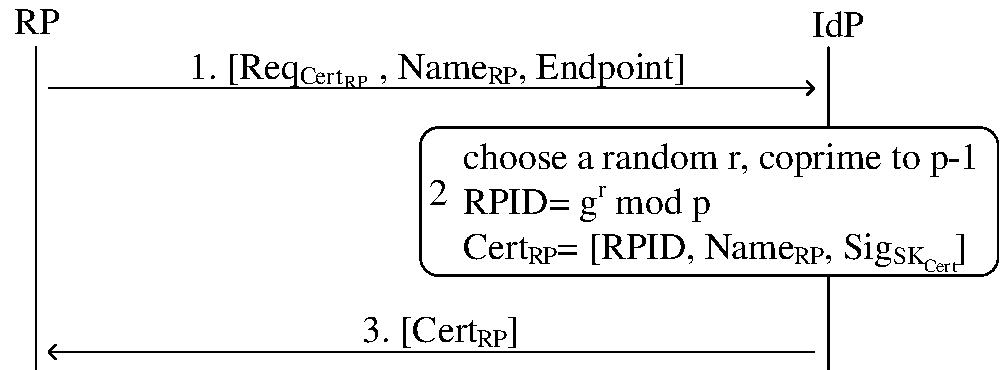
\includegraphics[width=\linewidth]{fig/registration.pdf}
  \caption{RP initial registration.}
  \label{fig:registration}
\end{figure}

%1. r which is coprime to $P-1$来保证$RPID$是一个本原根,从而保证adversary无法从PID中获取UID, ---
%2. $RPID$不能相同,保证RP无法进行identity linkage。 ---RP可以借助类似CT的方案来保证, 没有两个合法证书被颁发给同一个RPID
Here, we further explain the two requirements in the generation of $RPID$ for \textbf{Goal 4}:
\begin{itemize}
  \item $r$ should be coprime to $P-1$. This makes $RPID$ be another primitive root, and satisfies the requirement of Discrete Logarithm problem to prevent the RP  inferring $UID$ from $Account$.
  \item $r$ should be different with the ones for other RPs. Otherwise, the RPs who are assigned the same $RPID$, obtain the same PUID for a user, which makes identity linkage possible.
\end{itemize}

The honest IdP is assumed to generate the correct $RPID$. However, we may perform an external check on $Cert_{RP}$ and $RPID$, based on the idea of Certificate transparency. The external check needs to be performed by a third party instead of RP who will be able to perform identity linkage with incorrect $RPID$. To perform the external check, IdP is required to provide the $Cert_{RP}$ to a log server, while a monitor checks the correctness of $Cert_{RP}$, i.e., no two valid $Cert_{RP}$ assigned to a same $RPID$ and $RPID$ is a primitive root modulo $p$ as descried in Section~\ref{subsec:primitive}. Moreover, $Cert_{RP}$ is compatible with a X.509 certificate which is discussed in Section~\ref{sec:discussion}.
\end{comment}

\subsection{RP identifier transformation and Account calculation}
\label{subsec:identifier-generation}
In this section, we provide the calculation of $PRPID$, $PUID$ and $Account$ separately, which is the foundation of each user's login process described in Section~\ref{sebsec:loginprocess}.

{$PRPID$}. Similar to Diffie-Hellman key Exchange\cite{DiffieH76}, the RP and user generate the  $PRPID$ cooperatively as follows:
\begin{itemize}
  \item RP chooses a random odd number $n_{RP}$, and sends $Y_{RP} = {RPID}^{n_{RP}} mod \ p$ to the user.
  \item The user replies a random chosen odd number $n_{u}$ to the RP, and calculates $PRPID = {Y_{RP}}^{n_{u}} mod \ p$.
  \item RP also obtains $PRPID$ with the received $n_{u}$.
\end{itemize}

Therefore, $PRPID$ is denoted as Equation~\ref{equ:RPIDT}. The IdP fails to infer ${RPID}$ from $PRPID$ (\textbf{Privacy in Goal 2}).
   \begin{equation}
   PRPID = {Y_{RP}}^{n_{u}} = {RPID}^{n_{u}* n_{RP}} mod \ p
   \label{equ:RPIDT}
   \end{equation}

The generation ensures that $PRPID$ cannot be determined by neither (malicious) user nor RP, which prevents the adversary from constructing a identity proof to be accepted by two or more RPs (\textbf{Security in Goal 2}). RP fails to control the $PRPID$ generation, as it provides $Y_{RP}$ before obtaining $n_{u}$ and the modification of $Y_{RP}$ will trigger the user to generate another different  $n_{u}$. The Discrete Logarithm problem prevents the user from choosing a $n_{u}$ for a specified $PRPID$ on the received $Y_{RP}$.

Both $n_{RP}$ and $n_{u}$ are odd numbers, therefore $n_{RP}*n_{u}$ is an odd number and coprime to the even $p-1$, ensuring:
 \begin{itemize}
   \item $PRPID$ is a primite root modulo $p$, which prevents the RP from inferring $UID$ from $PUID$ (\textbf{Goal 4}).
   \item The inverse $(n_{RP}*n_{u})^{-1}$ exists, that is, $(n_{RP}*n_{u})^{-1} * (n_{RP}*n_{u}) = 1 \ mod \ (p-1)$. The inverse  serves as  the trapdoor $t$ for $Accout$, which makes:
   \begin{equation}
   (PRPID)^t = RPID \ mod \ p
   \label{equ:trapdoor}
   \end{equation}
 \end{itemize}

{$PUID$}. The IdP generates the $PUID$ based on the user's $UID$ and the user-provided $PRPID$, as denoted in Equation~\ref{equ:PUID}. $PUID$ varies for RPs due to the uniqueness of $PRPID$, satisfying \textbf{Goal 4}.
 \begin{equation}
   PUID = {PRPID}^{UID} \ mod \ p
   \label{equ:PUID}
   \end{equation}

{$Account$}. The RP calculates $PUID^t mod \ p$ as the  user's account, where $PUID$ is received from the user and $t$ is derived in the generation of $PRPID$. Equation~\ref{equ:account} demonstrates that $Account$ is unchanged to the RP during a user's multiple logins, satisfying \textbf{Goal 5}.
 \begin{equation}
   Account = ({PRPID}^{UID})^t = {RPID}^{UID} mod \ p
   \label{equ:account}
   \end{equation}


\subsection{User Login Process}
\label{sebsec:loginprocess}
In this section, we present the detailed process for each user's login as shown in Figure~\ref{fig:process}. The process corresponds to the goals 2-5 defined in Section~\ref{subsec:overview}.

\begin{figure*}
  \centering
  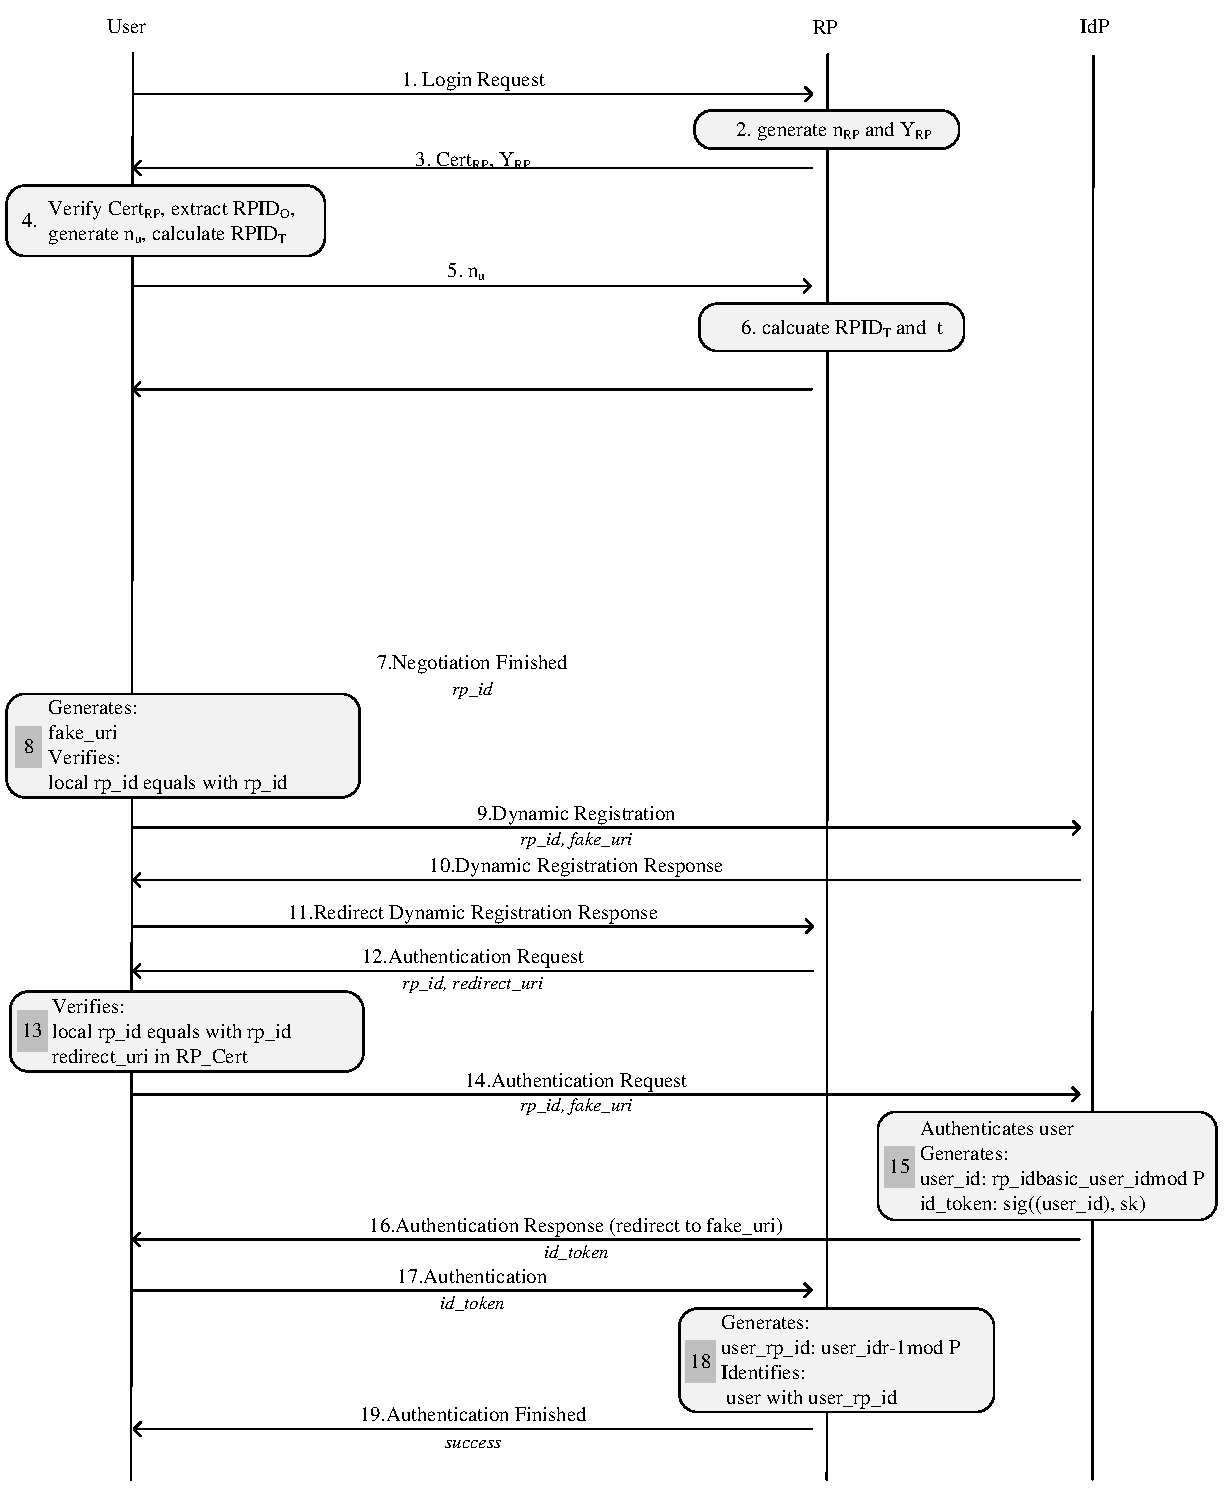
\includegraphics[width=0.85\linewidth]{fig/process.pdf}
  \caption{Process for each user's login.}
  \label{fig:process}
\end{figure*}

For RP identifer transforming, the user and RP corporately process as follows. \textbf{(1)} The user sends a login request to trigger the negotiation of $PRPID$. \textbf{(2)} RP chooses the random $n_{RP}$, and calculates $Y_{RP}$ as described in Section~\ref{subsec:identifier-generation}. \textbf{(3)} RP sends $Cert_{RP}$ with $Y_{RP}$ to the user.  \textbf{(4)} The user halts the login process if the provided $Cert_{RP}$ is invalid; otherwise, it extracts $RPID$ from $Cert_{RP}$, and calculates $PRPID$ with a random chosen $n_u$ as in Section~\ref{subsec:identifier-generation}. \textbf{(5)} The user sends $n_u$ and $PRPID$ to the RP. \textbf{(6)} RP calculates $PRPID$ using the received $n_u$ with $Y_{RP}$ as in Section~\ref{subsec:identifier-generation}, and rejects the user's login request if the calculated $PRPID$ is inconsistent with the received one. After that, RP derives the trapdoor $t$ as in Section~\ref{subsec:identifier-generation}, which will be used in calculating $Account$. \textbf{(7)} RP sends the calculated $PRPID$ to the user, who will halt the login if the received $PRPID$ is different from the cached one.

For dynamic registration, the user registers the RP at the IdP instead of RP as follows. \textbf{(8)} The user generates an one-time endpoint (used in Section~\ref{subsec:compatible}) if the received $PRPID$ is accepted. \textbf{(9)} Then, the user registers the RP with the $PRPID$ and one-time endpoint. \textbf{(10)} If $PRPID$ is globally unique and is a primitive root module $p$, IdP sets the flag $RegRes$ as $OK$ (otherwise $FAIL$), and constructs the reply in the form of
[$RegRes$, $RegMes$, $Sig_{SK_{ID}}$]
%[$RegRes$, $timestamp$, $PRPID$, $Sig_{SK_ID}$] where $timestamp$ is the time generating this reply and
where $RegMes$ is the response to traditional dynamic registration containing $PRPID$, issuing time with other attributes and $Sig_{SK_{ID}}$ is the signature of the other elements using the private key $SK_{ID}$ (satisfying \textbf{Goal 3}). \textbf{(11)} The user forwards the registering result to the RP. The user obtains $RegRes$ directly as the connection between the user and IdP is secure, while the RP accepts the $RegRes$ only when $Sig_{SK_{ID}}$ is valid
%, $timestamp$ is correct and $PRPID$ is the same as the cached one.
and $RegMes$ is issued for the $PRPID$ within the expiration date. The user and RP will negotiate a new $PRPID$ if $RegRes$ is $FAIL$.

To acquire the $PUID$, the user corporates with the RP and IdP as follows. \textbf{(12)} RP constructs an identity proof request with the correctly registered $PRPID$ and the endpoint (the form of the request is detailed in Section~\ref{subsec:compatible}). \textbf{(13)} The user halts the login process if the received $PRPID$ is different from the previous one. \textbf{(14)} The user replaces the endpoint with the registered one-time endpoint, and sends it with the identity proof request to the IdP. \textbf{(15)} IdP requires the user to provide the correct credentials if the user hasn't been unauthenticated; and rejects the request if the binding of $PRPID$ and the one-time endpoint doesn't exist in the registered ones. Then, IdP generates the $PUID$ as in Section~\ref{subsec:identifier-generation}, and constructs the identity proof with $PRPID$, $PUID$, the valid period, issuing time and other attribute values, by attaching a signature of these elements using the private key $SK_{ID}$. \textbf{(16)} IdP sends the identity proof with the one-time endpoint to the user. \textbf{(17)} The user forwards the identity proof to the RP's endpoint corresponding to the one-time endpoint.

Finally, RP derives the user's unchanged $Account$ from $PUID$ as follows. \textbf{(18)} RP accepts the identity proof only when the signature is correctly verified with $PK_{ID}$, $PRPID$ is the same as the negotiated one, the issuing time is less than current time, and the current time is in the validity period. If the identity proof is incorrect, RP returns login fail to the user who will trigger another login request. Otherwise, RP calculates the $Account$ as in Section~\ref{subsec:identifier-generation}. \textbf{(19)}, After obtaining the user's unchanged $Account$, RP sends the login result to the user and begins to provide the individual service.


\subsection{Compatibility with OIDC}
\label{subsec:compatible}
Recluse is compatible with the implicit protocol flow of OIDC (authorization code flow is discussed in Section~\ref{sec:discussion}).

In Recluse, the formats of identity proof request and identity proof are the same as the ones in OIDC. In details, each element of the identity proof request in OIDC is contained in Recluse as follows: the RP's identifier ($PRPID$ in Recluse), the endpoint (one-time endpoint in the request from the user in Recluse) and the set of required attributes (also supported by Recluse although not listed in the description). The identity proof in Recluse is also exactly the same as the one in OIDC, which includes RP's identifer ($PRPID$ in Recluse), the user's PPID ($PUID$ in Recluse), the issuer, validity period, issuing time, other requested attributes and a signature using the IdP's private key.

The same format of identity proof request and identity proof makes the verification same in OIDC and Recluse. The IdP, in both Recluse and OIDC, verifies the identity proof request, by checking whether the mapping of RP's identifier and endpoint exists in the registered ones. The RP, in both Recluse and OIDC, checks the correctness of identity proof, by checking that the signature is correct, the consistency of RP's identifer in the identity proof and the one it owns, the validity period, issuing time and the freshness (which is checked based on a nonce in  OIDC, while  $PRPID$ serves as the nonce in Recluse).

The RP's extra processes needed in Recluse may be achieved using the existing interfaces defined in OIDC.  Recluse requires that $PRPID$ is globally unique, which can be achieved through the dynamic registration (described in Section~\ref{sec:background}) provided by IdP in OIDC. In Recluse, the dynamic registration is invoked by the user instead of the RP to prevent the curious IdP infers the user's traces by analyzing the between the dynamic registration and identity proof request. To avoid the IdP to infer the RP's identity through the registration token in dynamic registration, the access control of the endpoint for dynamic registration is deleted in Recluse. As the registration response is transmitted through the user instead of server-to-server transmission between RP and IdP, the extra signature is required to guarantee the integrity of response. Moreover, the endpoint in the dynamic registration request is replaced with an one-time endpoint, to avoid the RP's identifying information to be leaked to the IdP.


The modification required by Recluse at the RP may be achieved using existing interface provided by the implementations of OIDC. Based on the software development kit (SDK) in existing OIDC implementations for RP, the Steps 2-3, 5-7, 12 (in Figure~\ref{fig:process}) in RP may be integrated in the interface for constructing identity proof request;
Step 18 in Figure~\ref{fig:process} may be combined with the interface for verifying and parsing identity proof.

The processes at the user may be achieved through an extension at the user agent, which captures the identity proof (and request) for process  without modifying existing message transmission at the IdP and RP (i.e., redirection mechanism), as described in Section~\ref{sec:implementation}.


Only the RP initial registration, step 10 and Step 15 in Figure~\ref{fig:process} requires a modification at IdP.

\begin{comment}
The overview of login flow is shown in Figure~\ref{fig:overview}, which contains RP identifier negotiation, dynamic registration and token obtaining.

The of each phase in login flow is shown as follows:
\begin{itemize}
\item[1.] RP Identifier Negotiation: The negotiation is required to generate the RP identifier. For each SSO procedure, user is going to start negotiation with user. RP identifier is a random number which does not represent any RP, generated by rp-id-generating algorithm. However, the identifier is bound with specific authentication which is able to be confirmed by user and RP. The details of identifier generation is shown in Section~\ref{sec:identifier-generation}.
\item[2.] Dynamic Registration: Dynamic registration is required to in Recluse to make sure the identifier generated by negotiation is valid in IdP. In OIDC system, RP should register its attributes (e.g., the endpoint for identity proof) with IdP and obtain the RP identifier generated by IdP so that IdP is able to authenticate the user for specific RP. Therefore, to make sure the newly generated RP identifier in RP Identifier Negotiation is valid in IdP, the dynamic registration is required before the authentication request is transmitted to IdP. IdP is to check whether the identifier is unique and require RP to restart identifier negotiation if the identifier has be used by another RP.
%To make the RP identifier generated by negotiation is valid in IdP, user is to register this identifier with IdP through the dynamic registration API provided by IdP. IdP is going to check whether the identifier is unique and require RP to restart identifier negotiation if the identifier has be used by another RP.
\item[3.] Authentication: After dynamic registration, RP builds the authentication request and redirects it to IdP through user agent. After receiving the request, IdP firstly authenticates user and then issues identity proof for RP, which contains the user id generated through the user-id-generating algorithm. Then IdP redirects the identity to RP through user agent, and RP identify the user through identity proof. The methods of user identifier generation and RP identifying the user are shown in Section~\ref{sec:identifier-generation}.
\end{itemize}

However, in addition to the login flow in each authentication, the initial registration is required before the RP and user integrates the Recluse service. The initial registration allows the RP to achieve the necessary parameters from the IdP and user to sign on in the IdP. In Recluse system, the initial registration is conducted by each RP and user only once, however, the login flow is conducted in each authentication integrally each time.



\subsection{Initial Registration}
The initial registration between RP and IdP is shown as Figure~\ref{fig:registration}.
\begin{figure}
  \centering
  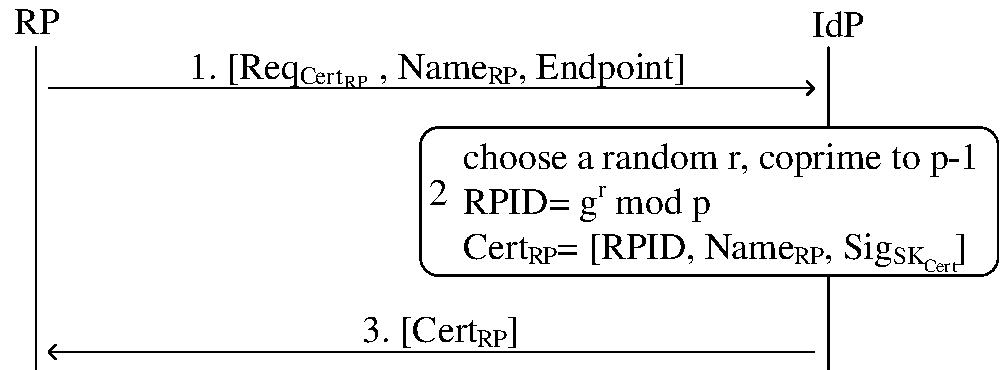
\includegraphics[width=\linewidth]{fig/registration.pdf}
  \caption{Prior Registration}
  \label{fig:registration}
\end{figure}
The registration process is as follows:
\begin{itemize}
\item[1.] Uploading Attributes: Firstly, IdP generates its prime $p$, the primitive root $g$ of $p$, used for RP and user identifier generation and the key pair $pk$, $sk$.
\item[2.]The RP uploads it attributes, such as its name, endpoint, identity proof (e.g., business license) and so on.
\item[3.] Issuing RP Certification: IdP verifies the identity of RP and generates the RP certification including $basic\_rp\_id$, $rp\_name$, \verb+redirect_uri+ and \verb+IdP_origin+.  The RP certification is used for user agent to verify the basic attributes, such as $basic\_rp\_id$ and \verb+redirect_uri+.
\item[4.]IdP returns the RP certification, $p$, $g$ and $pk$ to RP.
\end{itemize}

The initial registration required for IdP to verify the basic attributes of RP, such as name, endpoints for identity proof, so that Idp is able to provide the RP certification to RP which includes the unique identifier for each RP and its attributes. With the RP certification, user agent has the ability to verify the RP's endpoint for identity proof and notify user with RP's identity. Additionally, the parameters, prime $p$ (used for user id generating) with its primitive root $g$, public key of IdP $pk$ is provided in registration as well.
Same as RP, user need to register with IdP and IdP generates unique user id for each user.



\subsection{Rp-id-generating and User-id-generating algorithm}
\label{subsec:identifier-generation}
The rp-id-generating and user-id-generating algorithm are created based on Discrete Logarithm problem\cite{shiu2007cryptography:}.
IdP carefully chooses a big prime $p$\footnotetext[1]{$p$ is generated as $P=q\cdot 2+1$, while $q$ is prime as well.} and its primitive root \verb+g+ as generator for system. When the RP registers with IdP, IdP provides a unique primitive root as the RP's root identifier (called $basic_rp_id$).

For each login process, the user and RP negotiate the temporary RP identifier bound with specific authentication.
\subsubsection{$rp\_id$ generating}
While starting a login procedure, there is Diffie-Hellman key Exchange\cite{DiffieH76} between RP and user, through which the random $r$ is generated. However, to make sure that there is $r^{-1}$, that $r\cdot r^{-1}=1 mod \phi(P)$, $r$ should be the relative prime of $\phi(P)$, so that if $r$ is even $r$ should be added by one. Although there is little possibility that $r$ is the multiple of $p$ or $q$, it is not considered in the illustration. However, the re-negotiation is required in the practical system if $r$ is the multiple of $p$ or $q$. The RP identifier is generated as:
$$rp\_id=basic\_rp\_id^r mod P\eqno(1)$$
such that $rp_id$ is another primitive element module $p$. And $r^{-1}$ is generated through Extended Euclidean algorithm.
\subsubsection{$user\_id$ generating}
IdP labels each user at IdP with the unique identifier called $baisc\_user\_id$. To generate the specific user identifier for each $rp\_id$, the algorithm is
$$user\_id=rp\_id^{basic\_user\_id} mod P\eqno(2)$$
so
$$user\_id=basic\_rp\_id^{r\cdot basic\_user\_id}modP\eqno(3)$$
\subsubsection{Trapdoor}
While receiving $user\_id$ from IdP, RP is able to derive the constant user identifier from if
$$user\_rp\_id=user\_id^{r^{-1}} mod P\eqno(4)$$
so
$$user\_rp\_id=basic\_rp\_id^{(1 mod \phi(P))\cdot basic\_user\_id} mod P\eqno(5)$$
so
$$user\_rp\_id=basic\_rp\_id^{basic\_user\_id} mod P\eqno(6)$$
For single user in a RP, $user\_rp\_id$ is unchanged. However, $user\_rp\_id$s are distinct in each RP because $basic\_rp\_id$s are different in each RP.



\subsection{User Login Process}
\label{sebsec:loginprocess}
The login flow is shown as Figure~\ref{fig:process}, in which the $rp\_id$ is generated in step 6, the $user\_id$ is generated in step 15 and the RP derives the $user\_rp\_id$ in step 18.
\begin{figure*}
  \centering
  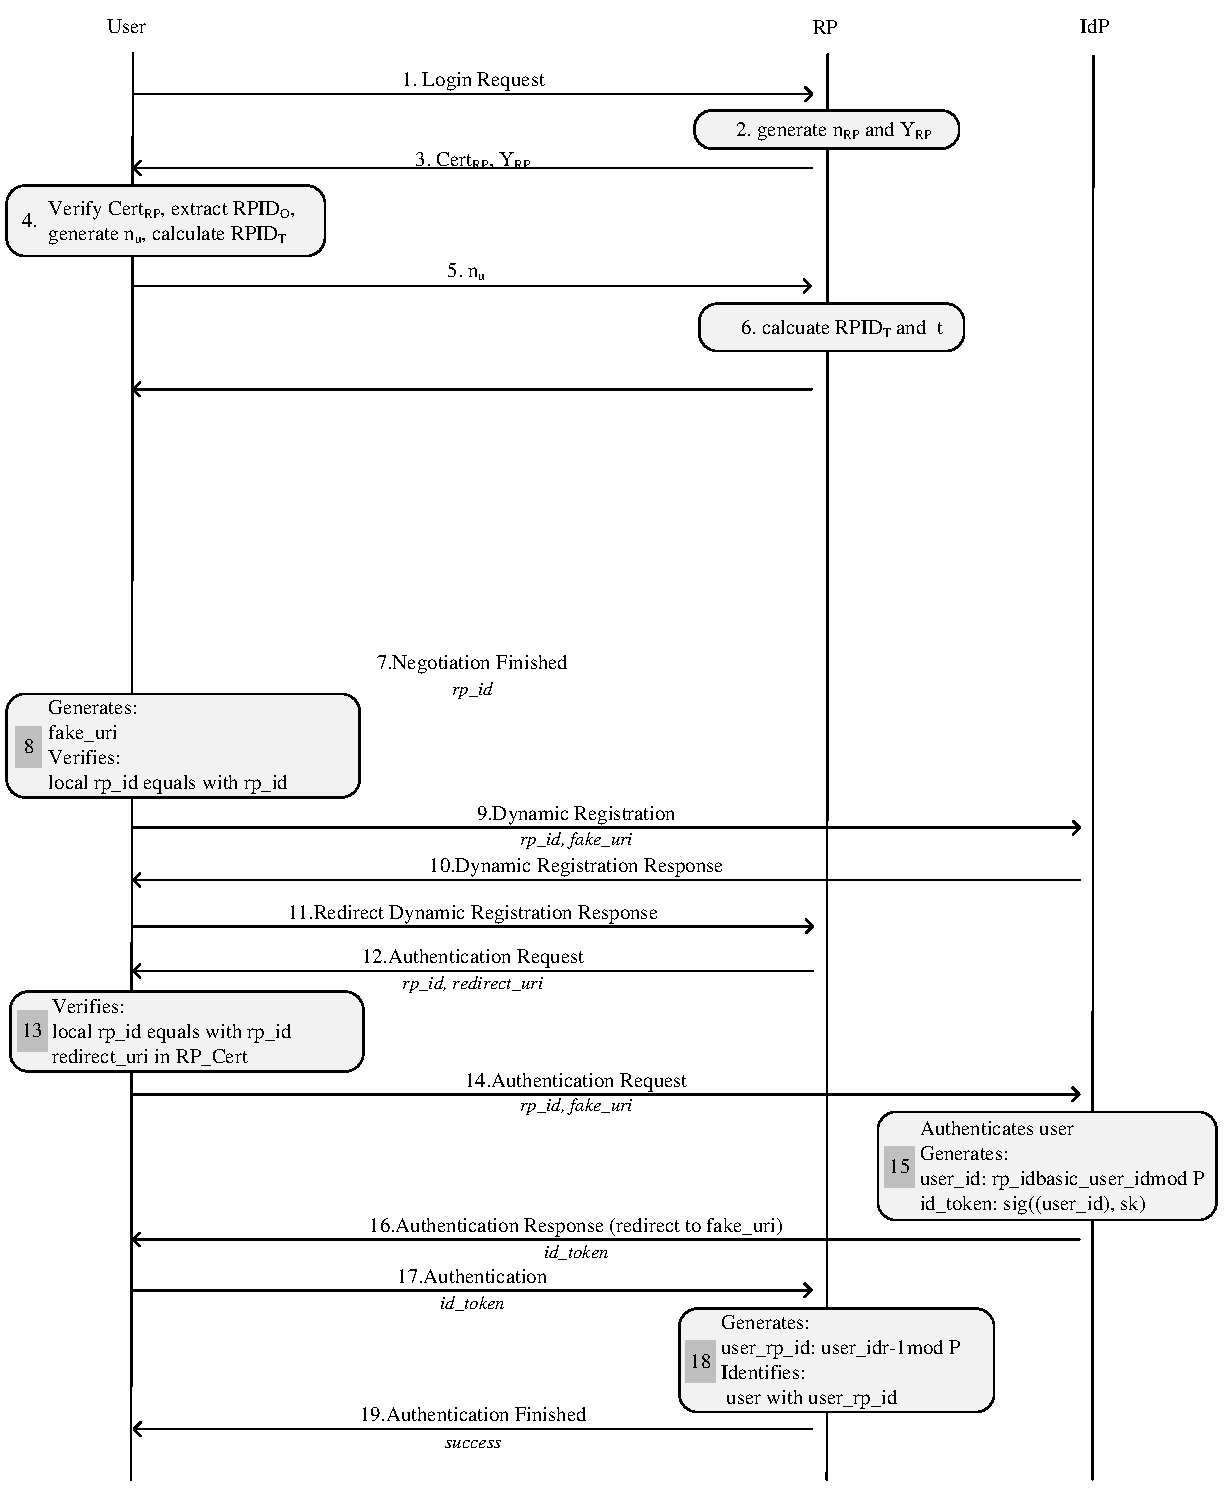
\includegraphics[width=\linewidth]{fig/process.pdf}
  \caption{Login Flow}
  \label{fig:process}
\end{figure*}

%抵抗phishing攻击:一定需要正确的RP参与,攻击者作为中间人
%1.使用IdP提供应用basic_rp_id与url的绑定,user agent保存映射
%缺点:占用空间,user agent需要缓存整个映射
%2.RP与用户通过加密的通道传输redirect_uri

%如果由RP选择basic_rp_id,那么多个rp之间的basic_rp_id有幂次关系,那么就可以关联用户

\subsubsection{RP Identifier Negotiation}
RP identifier negotiation starts form step 1 to step 7. The user accesses the service provided by RP in his/her browser. To log in this RP, user needs to click the login button offered by Recluse.
Firstly, the user agent sends the \verb+Start Negotiation+ request to RP, so that RP generates the random $sk\_rp$ and $pk\_rp=g^{sk\_rp}modP$ as the private key and public key for DH Key exchanging.
Secondly, RP builds the \verb+Negotiation Response+ with newly generated $pk\_rp$ as well as the \verb+RP_Cert+ issued by IdP. User agent similarly generates random $sk\_user$ and $pk\_user$, and $r=pk\_rp^{sk\_user}modP$. However, to make sure that $r$ is the relative prime of $\phi(P)$, it is required that $r$ should be odd and the greatest common divisor of $r$ and $\phi(P)$ is 1.
Then user agent continues the \verb+Negotiation+ sending $pk\_user$ and $r$ to RP. RP generates the local $r$ in the same way as user agent and compares the local $r$ and user agent generated $r$. If $r$s are equal, RP generates $rp\_id=basic\_rp\_id^rmodP$, as well as $r^{-1}$ through Extend Euclidean algorithm, which meets $r\cdot r^{-1}=1mod\phi(P)$.
Finally RP transmits the $rp\_id$ to user agent.
\subsubsection{Dynamic Registration}
Dynamic registration is from step 8 to step 13. While user agent receives teh $rp\_id$ from RP, it is required the $rp\_id$ from RP should be equal with it generated by user agent. Then user agent generates the \verb+fake_uri+ which contains the random string and keeps it for further identity proof transmission. User agent sends the \verb+Dynamic Registration+ request to IdP with newly generated $rp\_id$ and \verb+fake_uri+ and redirects the \verb+Dynamic Registration Response+ to RP.
\subsubsection{Authentication}
Authentication is from step 14 to step 19. After dynamic registration,  RP builds the \verb+Authentication Request+ including $rp\_id$ as well as the \verb+redirect_uri+ representing the endpoint, and redirects it to IdP through user agent. User agent tampers the authentication request, compares $rp\_id$ with the local one, verifies the validation of the \verb+redirect_uri+ and replaces it with the fake one. Then user agent transmits the \verb+Authentication Request+ to IdP. After receiving the request, IdP firstly authenticates user and then generates $user\_id=rp\_id^{basic\_user\_id}modP$. The identity proof signed with IdP's private key including the $user\_id$ is redirected to the \verb+fake_uri+ through user agent, who intercepts the transmission and transmit it to the endpoint \verb+redirect_uri+ in authentication request. Finally, RP derives the constant $user\_rp\_id$ from $user\_id$. If the $user\_rp\_id$ has already been registered, RP send \verb+Authentication Finished+ with the message \verb+success+ to user agent.

%描述user_id, rp_id and user_rp_id的生成
\end{comment}
